% Options for packages loaded elsewhere
\PassOptionsToPackage{unicode}{hyperref}
\PassOptionsToPackage{hyphens}{url}
%
\documentclass[
  ignorenonframetext,
]{beamer}
\usepackage{pgfpages}
\setbeamertemplate{caption}[numbered]
\setbeamertemplate{caption label separator}{: }
\setbeamercolor{caption name}{fg=normal text.fg}
\beamertemplatenavigationsymbolsempty
% Prevent slide breaks in the middle of a paragraph
\widowpenalties 1 10000
\raggedbottom
\setbeamertemplate{part page}{
  \centering
  \begin{beamercolorbox}[sep=16pt,center]{part title}
    \usebeamerfont{part title}\insertpart\par
  \end{beamercolorbox}
}
\setbeamertemplate{section page}{
  \centering
  \begin{beamercolorbox}[sep=12pt,center]{part title}
    \usebeamerfont{section title}\insertsection\par
  \end{beamercolorbox}
}
\setbeamertemplate{subsection page}{
  \centering
  \begin{beamercolorbox}[sep=8pt,center]{part title}
    \usebeamerfont{subsection title}\insertsubsection\par
  \end{beamercolorbox}
}
\AtBeginPart{
  \frame{\partpage}
}
\AtBeginSection{
  \ifbibliography
  \else
    \frame{\sectionpage}
  \fi
}
\AtBeginSubsection{
  \frame{\subsectionpage}
}
\usepackage{amsmath,amssymb}
\usepackage{lmodern}
\usepackage{iftex}
\ifPDFTeX
  \usepackage[T1]{fontenc}
  \usepackage[utf8]{inputenc}
  \usepackage{textcomp} % provide euro and other symbols
\else % if luatex or xetex
  \usepackage{unicode-math}
  \defaultfontfeatures{Scale=MatchLowercase}
  \defaultfontfeatures[\rmfamily]{Ligatures=TeX,Scale=1}
\fi
% Use upquote if available, for straight quotes in verbatim environments
\IfFileExists{upquote.sty}{\usepackage{upquote}}{}
\IfFileExists{microtype.sty}{% use microtype if available
  \usepackage[]{microtype}
  \UseMicrotypeSet[protrusion]{basicmath} % disable protrusion for tt fonts
}{}
\makeatletter
\@ifundefined{KOMAClassName}{% if non-KOMA class
  \IfFileExists{parskip.sty}{%
    \usepackage{parskip}
  }{% else
    \setlength{\parindent}{0pt}
    \setlength{\parskip}{6pt plus 2pt minus 1pt}}
}{% if KOMA class
  \KOMAoptions{parskip=half}}
\makeatother
\usepackage{xcolor}
\newif\ifbibliography
\usepackage{color}
\usepackage{fancyvrb}
\newcommand{\VerbBar}{|}
\newcommand{\VERB}{\Verb[commandchars=\\\{\}]}
\DefineVerbatimEnvironment{Highlighting}{Verbatim}{commandchars=\\\{\}}
% Add ',fontsize=\small' for more characters per line
\usepackage{framed}
\definecolor{shadecolor}{RGB}{248,248,248}
\newenvironment{Shaded}{\begin{snugshade}}{\end{snugshade}}
\newcommand{\AlertTok}[1]{\textcolor[rgb]{0.94,0.16,0.16}{#1}}
\newcommand{\AnnotationTok}[1]{\textcolor[rgb]{0.56,0.35,0.01}{\textbf{\textit{#1}}}}
\newcommand{\AttributeTok}[1]{\textcolor[rgb]{0.77,0.63,0.00}{#1}}
\newcommand{\BaseNTok}[1]{\textcolor[rgb]{0.00,0.00,0.81}{#1}}
\newcommand{\BuiltInTok}[1]{#1}
\newcommand{\CharTok}[1]{\textcolor[rgb]{0.31,0.60,0.02}{#1}}
\newcommand{\CommentTok}[1]{\textcolor[rgb]{0.56,0.35,0.01}{\textit{#1}}}
\newcommand{\CommentVarTok}[1]{\textcolor[rgb]{0.56,0.35,0.01}{\textbf{\textit{#1}}}}
\newcommand{\ConstantTok}[1]{\textcolor[rgb]{0.00,0.00,0.00}{#1}}
\newcommand{\ControlFlowTok}[1]{\textcolor[rgb]{0.13,0.29,0.53}{\textbf{#1}}}
\newcommand{\DataTypeTok}[1]{\textcolor[rgb]{0.13,0.29,0.53}{#1}}
\newcommand{\DecValTok}[1]{\textcolor[rgb]{0.00,0.00,0.81}{#1}}
\newcommand{\DocumentationTok}[1]{\textcolor[rgb]{0.56,0.35,0.01}{\textbf{\textit{#1}}}}
\newcommand{\ErrorTok}[1]{\textcolor[rgb]{0.64,0.00,0.00}{\textbf{#1}}}
\newcommand{\ExtensionTok}[1]{#1}
\newcommand{\FloatTok}[1]{\textcolor[rgb]{0.00,0.00,0.81}{#1}}
\newcommand{\FunctionTok}[1]{\textcolor[rgb]{0.00,0.00,0.00}{#1}}
\newcommand{\ImportTok}[1]{#1}
\newcommand{\InformationTok}[1]{\textcolor[rgb]{0.56,0.35,0.01}{\textbf{\textit{#1}}}}
\newcommand{\KeywordTok}[1]{\textcolor[rgb]{0.13,0.29,0.53}{\textbf{#1}}}
\newcommand{\NormalTok}[1]{#1}
\newcommand{\OperatorTok}[1]{\textcolor[rgb]{0.81,0.36,0.00}{\textbf{#1}}}
\newcommand{\OtherTok}[1]{\textcolor[rgb]{0.56,0.35,0.01}{#1}}
\newcommand{\PreprocessorTok}[1]{\textcolor[rgb]{0.56,0.35,0.01}{\textit{#1}}}
\newcommand{\RegionMarkerTok}[1]{#1}
\newcommand{\SpecialCharTok}[1]{\textcolor[rgb]{0.00,0.00,0.00}{#1}}
\newcommand{\SpecialStringTok}[1]{\textcolor[rgb]{0.31,0.60,0.02}{#1}}
\newcommand{\StringTok}[1]{\textcolor[rgb]{0.31,0.60,0.02}{#1}}
\newcommand{\VariableTok}[1]{\textcolor[rgb]{0.00,0.00,0.00}{#1}}
\newcommand{\VerbatimStringTok}[1]{\textcolor[rgb]{0.31,0.60,0.02}{#1}}
\newcommand{\WarningTok}[1]{\textcolor[rgb]{0.56,0.35,0.01}{\textbf{\textit{#1}}}}
\usepackage{graphicx}
\makeatletter
\def\maxwidth{\ifdim\Gin@nat@width>\linewidth\linewidth\else\Gin@nat@width\fi}
\def\maxheight{\ifdim\Gin@nat@height>\textheight\textheight\else\Gin@nat@height\fi}
\makeatother
% Scale images if necessary, so that they will not overflow the page
% margins by default, and it is still possible to overwrite the defaults
% using explicit options in \includegraphics[width, height, ...]{}
\setkeys{Gin}{width=\maxwidth,height=\maxheight,keepaspectratio}
% Set default figure placement to htbp
\makeatletter
\def\fps@figure{htbp}
\makeatother
\setlength{\emergencystretch}{3em} % prevent overfull lines
\providecommand{\tightlist}{%
  \setlength{\itemsep}{0pt}\setlength{\parskip}{0pt}}
\setcounter{secnumdepth}{-\maxdimen} % remove section numbering
\ifLuaTeX
  \usepackage{selnolig}  % disable illegal ligatures
\fi
\IfFileExists{bookmark.sty}{\usepackage{bookmark}}{\usepackage{hyperref}}
\IfFileExists{xurl.sty}{\usepackage{xurl}}{} % add URL line breaks if available
\urlstyle{same} % disable monospaced font for URLs
\hypersetup{
  pdftitle={Visualization of networks and communities},
  pdfauthor={Fabio Morea},
  hidelinks,
  pdfcreator={LaTeX via pandoc}}

\title{Visualization of networks and communities}
\author{Fabio Morea}
\date{2023-05-13}

\begin{document}
\frame{\titlepage}

\begin{frame}{introduction}
\protect\hypertarget{introduction}{}
\begin{block}{Networks and communities}
\protect\hypertarget{networks-and-communities}{}
Network analysis is a powerful tool for understanding complex systems in
both the hard and social sciences. By representing data as a network, it
is possible to identify communities of similar members, or nodes, that
are connected to each other by various relationships.

This allows to gain insights into the structure of the system, as well
as the behavior of the nodes within it.

\emph{For example, in social networks, nodes can represent people, and
the relationships between them can represent various types of
interactions, such as friendships or collaborations. By analyzing the
network, researchers can identify clusters of people who are more likely
to interact with each other, or who share similar characteristics.}
\end{block}

\begin{block}{Networks and communities: a toy example}
\protect\hypertarget{networks-and-communities-a-toy-example}{}
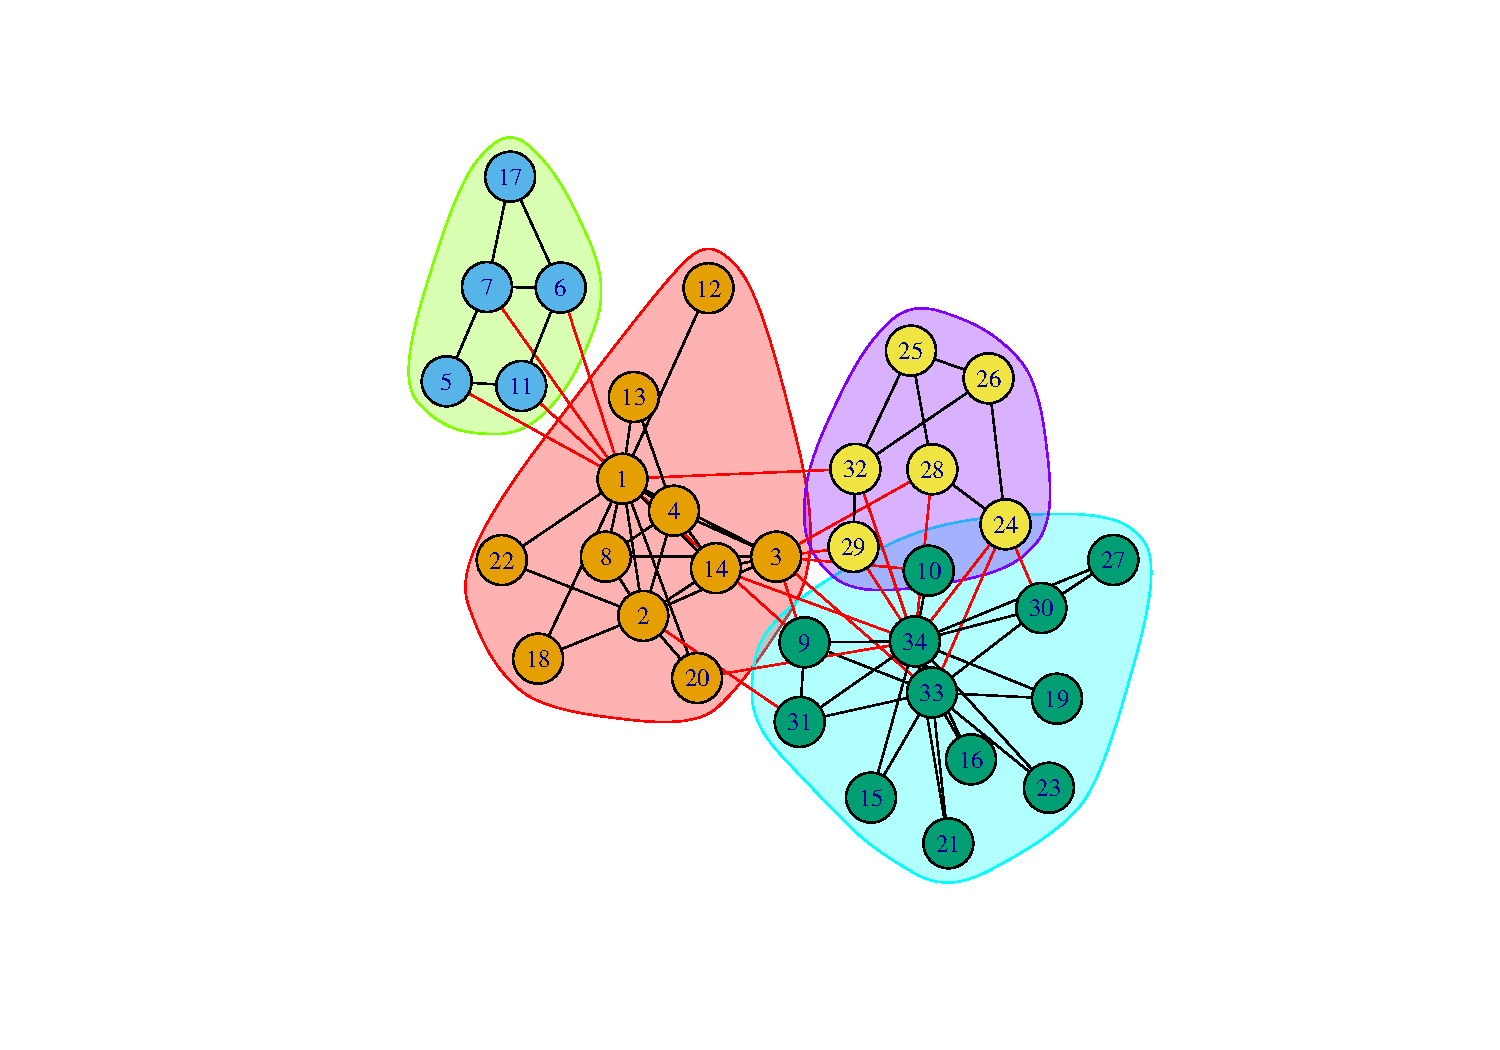
\includegraphics{presentation1_files/figure-beamer/unnamed-chunk-2-1.pdf}
\end{block}

\begin{block}{Communities in large networks}
\protect\hypertarget{communities-in-large-networks}{}
As the size of a network increases, the complexity of the network also
increases, making it difficult to represent the network in a simple
visual format. As a result, a simple visualization may not provide much
clarity in understanding the structure of the network. To gain a better
understanding of a large network, more sophisticated visualizations and
analysis techniques are needed.
\end{block}

\begin{block}{Contents of this seminar}
\protect\hypertarget{contents-of-this-seminar}{}
\begin{enumerate}
\item
  A family of benchmark networks (with built-in communities and
  controlled \emph{fuzzyness})
\item
  Visualization of network and communities (standard and custom layouts,
  k-core VS strength)
\item
  Modularity-based community detection
\item
  robustness of results in \emph{fuzzy} networks
\item
  consensus and ``robustness of membership''
\item
  sample results in a ``labour market network''
\end{enumerate}
\end{block}
\end{frame}

\begin{frame}[fragile]{1 A family of benchmark networks (with built-in
communities and controlled \emph{fuzzyness})}
\protect\hypertarget{a-family-of-benchmark-networks-with-built-in-communities-and-controlled-fuzzyness}{}
\begin{block}{About LFR benchmark networks}
\protect\hypertarget{about-lfr-benchmark-networks}{}
LFR (Lancichinetti-Fortunato-Radicchi) benchmark graphs are synthetic
networks used to evaluate the performance of network analysis
algorithms. They are generated using a stochastic block model and are
designed to have realistic community structure, degree distributions,
and other properties of real-world networks.

They are used to test the accuracy of algorithms for network analysis
tasks such as community detection, link prediction, and node
classification.

Benchmark graphs for testing community detection algorithms, Andrea
Lancichinetti, Santo Fortunato, and Filippo Radicchi, Phys. Rev.~E 78,
046110 2008

\href{https://networkx.org/documentation/stable/reference/generated/networkx.generators.community.LFR_benchmark_graph.html}{LFR\_benchmark\_graph
--- NetworkX 3.1 documentation}
\end{block}

\begin{block}{Building a family of LFR benchmark networks}
\protect\hypertarget{building-a-family-of-lfr-benchmark-networks}{}
in Python , networkx LFR\_benchmark\_graph()
\href{https://networkx.org/documentation/stable/reference/generated/networkx.generators.community.LFR_benchmark_graph.html}{\emph{https://networkx.org/documentation/stable/reference/generated/networkx.generators.community.LFR\_benchmark\_graph.html}}

\begin{Shaded}
\begin{Highlighting}[]
\ControlFlowTok{for}\NormalTok{ mui }\KeywordTok{in} \BuiltInTok{range}\NormalTok{(}\DecValTok{10}\NormalTok{,}\DecValTok{99}\NormalTok{,}\DecValTok{20}\NormalTok{):}
    \BuiltInTok{print}\NormalTok{(}\StringTok{"generating LFR benchmark. Fuzzyness mu = "}\NormalTok{, mui}\OperatorTok{/}\DecValTok{100}\NormalTok{)}
\NormalTok{    gb }\OperatorTok{=}\NormalTok{ LFR\_benchmark\_graph( mu}\OperatorTok{=}\NormalTok{mui}\OperatorTok{/}\DecValTok{100}\NormalTok{, }
\NormalTok{        n}\OperatorTok{=} \DecValTok{250}\NormalTok{,  }
\NormalTok{        tau1 }\OperatorTok{=} \DecValTok{2}\NormalTok{, }
\NormalTok{        tau2 }\OperatorTok{=} \DecValTok{2}\NormalTok{, }
\NormalTok{        average\_degree}\OperatorTok{=}\DecValTok{5}\NormalTok{, }
\NormalTok{        min\_community}\OperatorTok{=}\DecValTok{30}\NormalTok{, }
\NormalTok{        seed}\OperatorTok{=}\DecValTok{42}\NormalTok{)}
\NormalTok{    gt }\OperatorTok{=}\NormalTok{ add\_true\_labels(gb)}
\NormalTok{    nx.write\_gml(gt, }\SpecialStringTok{f"./LFR\_graphs/small/FLR\_benchmark\_}\SpecialCharTok{\{}\NormalTok{mui}\SpecialCharTok{\}}\SpecialStringTok{.gml"}\NormalTok{)}
\end{Highlighting}
\end{Shaded}

\begin{verbatim}
## generating LFR benchmark. Fuzzyness mu =  0.1
## generating LFR benchmark. Fuzzyness mu =  0.3
## generating LFR benchmark. Fuzzyness mu =  0.5
## generating LFR benchmark. Fuzzyness mu =  0.7
## generating LFR benchmark. Fuzzyness mu =  0.9
\end{verbatim}
\end{block}
\end{frame}

\begin{frame}[fragile]{2- Visualization of network and communities
(standard and custom layouts, k-core VS strength)}
\protect\hypertarget{visualization-of-network-and-communities-standard-and-custom-layouts-k-core-vs-strength}{}
\begin{block}{print mu = 10\%}
\protect\hypertarget{print-mu-10}{}
\ldots{}

\begin{verbatim}
## [1] "Loading graph... ./LFR_graphs/small/FLR_benchmark_10.gml"
\end{verbatim}

\begin{verbatim}
##             [,1]       [,2]
##  [1,] -5.5778662  3.9127641
##  [2,] -7.6868497  4.9849037
##  [3,]  4.9864714  5.5796091
##  [4,] -4.5890687 -6.5865647
##  [5,]  6.7984379  7.0346978
##  [6,]  0.8311986 -9.8203107
##  [7,]  3.7517526 10.2162907
##  [8,] -5.2538770 -0.7669972
##  [9,] -6.5424370  9.0386186
## [10,] -5.0918284 12.3526960
\end{verbatim}
\end{block}

\begin{block}{plot function}
\protect\hypertarget{plot-function}{}
\begin{Shaded}
\begin{Highlighting}[]
\NormalTok{plot\_graph\_and\_comms }\OtherTok{\textless{}{-}} \ControlFlowTok{function}\NormalTok{(mui , }\AttributeTok{show\_comms =} \ConstantTok{TRUE}\NormalTok{) \{}
\NormalTok{  filename }\OtherTok{=} \FunctionTok{paste0}\NormalTok{(}\StringTok{"./LFR\_graphs/small/FLR\_benchmark\_"}\NormalTok{, mui, }\StringTok{".gml"}\NormalTok{)}
  \FunctionTok{print}\NormalTok{(}\FunctionTok{paste}\NormalTok{(}\StringTok{"Benchmark network "}\NormalTok{, filename,}\StringTok{"and communities (true{-}labels)"}\NormalTok{))}
\NormalTok{  g }\OtherTok{\textless{}{-}} \FunctionTok{read\_graph}\NormalTok{(filename, }\AttributeTok{format =} \StringTok{"gml"}\NormalTok{)}
\NormalTok{  LO }\OtherTok{=} \FunctionTok{layout\_with\_fr}\NormalTok{(g)}
  \ControlFlowTok{if}\NormalTok{ (show\_comms }\SpecialCharTok{==} \ConstantTok{TRUE}\NormalTok{) \{}
\NormalTok{    comms }\OtherTok{=} \FunctionTok{table}\NormalTok{(}\FunctionTok{V}\NormalTok{(g)}\SpecialCharTok{$}\NormalTok{community)}
\NormalTok{    comms }\OtherTok{=} \FunctionTok{make\_clusters}\NormalTok{(g,}
                          \AttributeTok{membership =} \FunctionTok{V}\NormalTok{(g)}\SpecialCharTok{$}\NormalTok{community,}
                          \AttributeTok{modularity =} \ConstantTok{FALSE}\NormalTok{)}
    \FunctionTok{plot}\NormalTok{(}
\NormalTok{      comms,}
\NormalTok{      g,}
      \AttributeTok{vertex.color =} \FunctionTok{V}\NormalTok{(g)}\SpecialCharTok{$}\NormalTok{community,}
      \AttributeTok{layout =}\NormalTok{ LO,}
      \AttributeTok{vertex.size =} \DecValTok{5}\NormalTok{,}
      \AttributeTok{vertex.label =} \ConstantTok{NA}
\NormalTok{    )}
\NormalTok{  \} }\ControlFlowTok{else}\NormalTok{ \{}
    \FunctionTok{plot}\NormalTok{(}
\NormalTok{      g,}
      \AttributeTok{vertex.color =} \FunctionTok{V}\NormalTok{(g)}\SpecialCharTok{$}\NormalTok{community,}
      \AttributeTok{layout =}\NormalTok{ LO,}
      \AttributeTok{vertex.size =} \DecValTok{5}\NormalTok{,}
      \AttributeTok{vertex.label =} \ConstantTok{NA}
\NormalTok{    )}
    
\NormalTok{  \}}
  \FunctionTok{return}\NormalTok{(}\DecValTok{1}\NormalTok{)}
\NormalTok{\}}
\end{Highlighting}
\end{Shaded}
\end{block}

\begin{block}{sample network ( mu = 0.10 )}
\protect\hypertarget{sample-network-mu-0.10}{}
\begin{Shaded}
\begin{Highlighting}[]
\FunctionTok{plot\_graph\_and\_comms}\NormalTok{(}\AttributeTok{mui =} \DecValTok{10}\NormalTok{ , }\AttributeTok{show\_comms =} \ConstantTok{FALSE}\NormalTok{) }
\end{Highlighting}
\end{Shaded}

\begin{verbatim}
## [1] "Benchmark network  ./LFR_graphs/small/FLR_benchmark_10.gml and communities (true-labels)"
\end{verbatim}

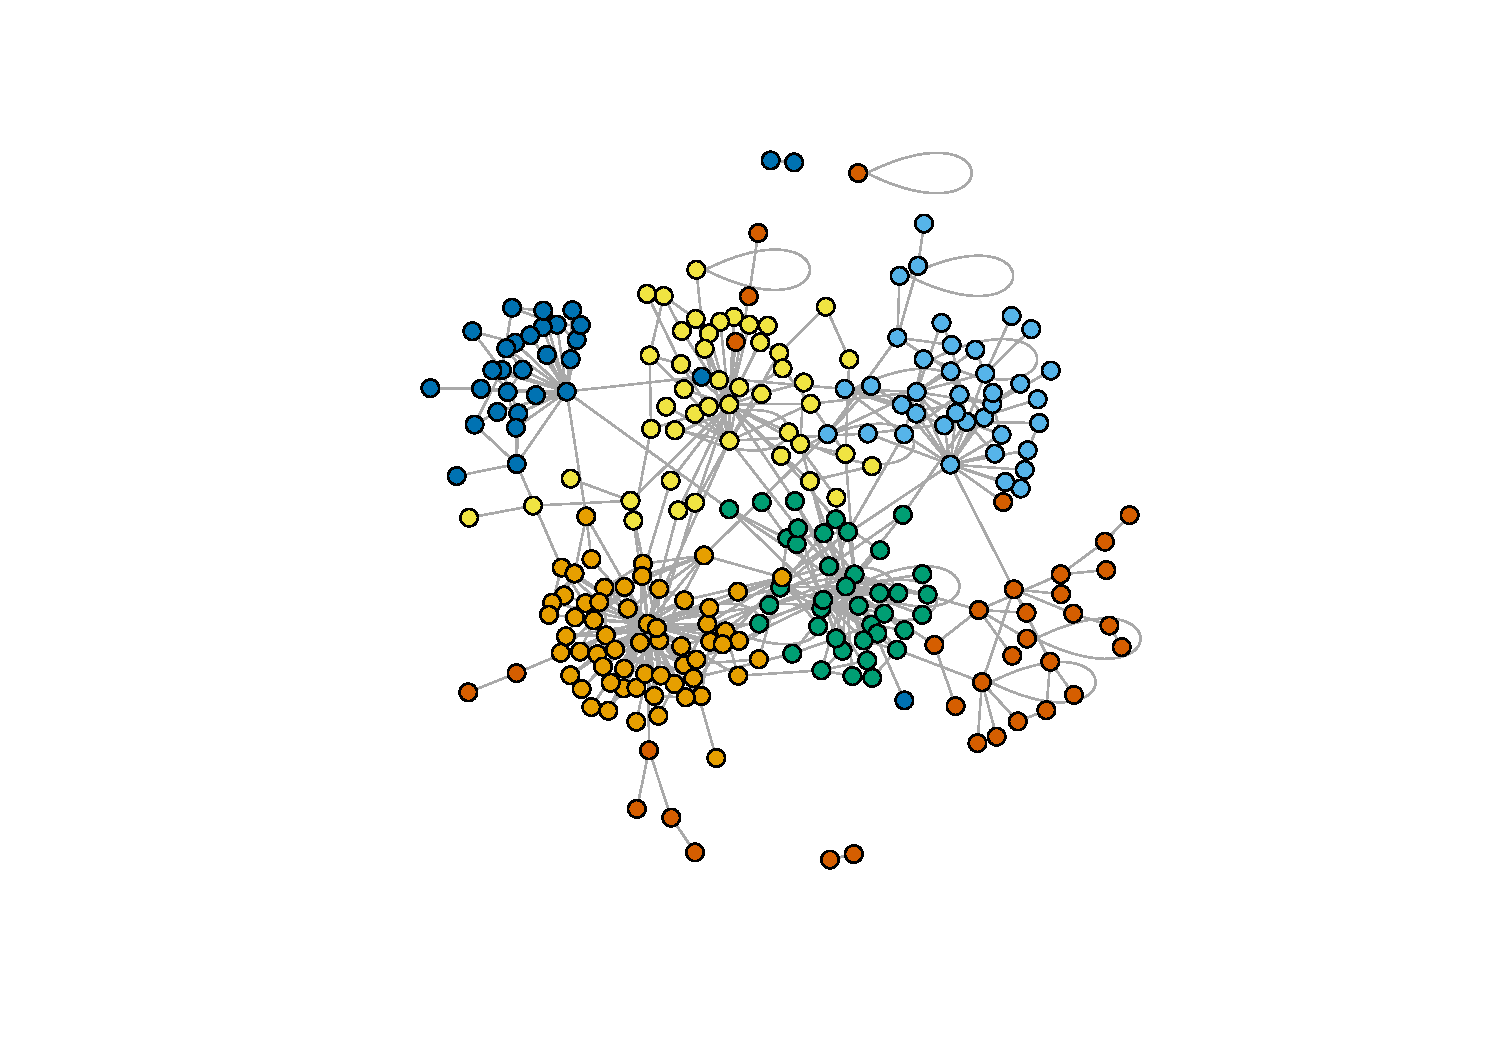
\includegraphics{presentation1_files/figure-beamer/unnamed-chunk-9-1.pdf}

\begin{verbatim}
## [1] 1
\end{verbatim}
\end{block}

\begin{block}{sample network ( mui = 0.50 )}
\protect\hypertarget{sample-network-mui-0.50}{}
\begin{Shaded}
\begin{Highlighting}[]
\FunctionTok{plot\_graph\_and\_comms}\NormalTok{(}\AttributeTok{mui =} \DecValTok{50}\NormalTok{ , }\AttributeTok{show\_comms =} \ConstantTok{FALSE}\NormalTok{) }
\end{Highlighting}
\end{Shaded}

\begin{verbatim}
## [1] "Benchmark network  ./LFR_graphs/small/FLR_benchmark_50.gml and communities (true-labels)"
\end{verbatim}

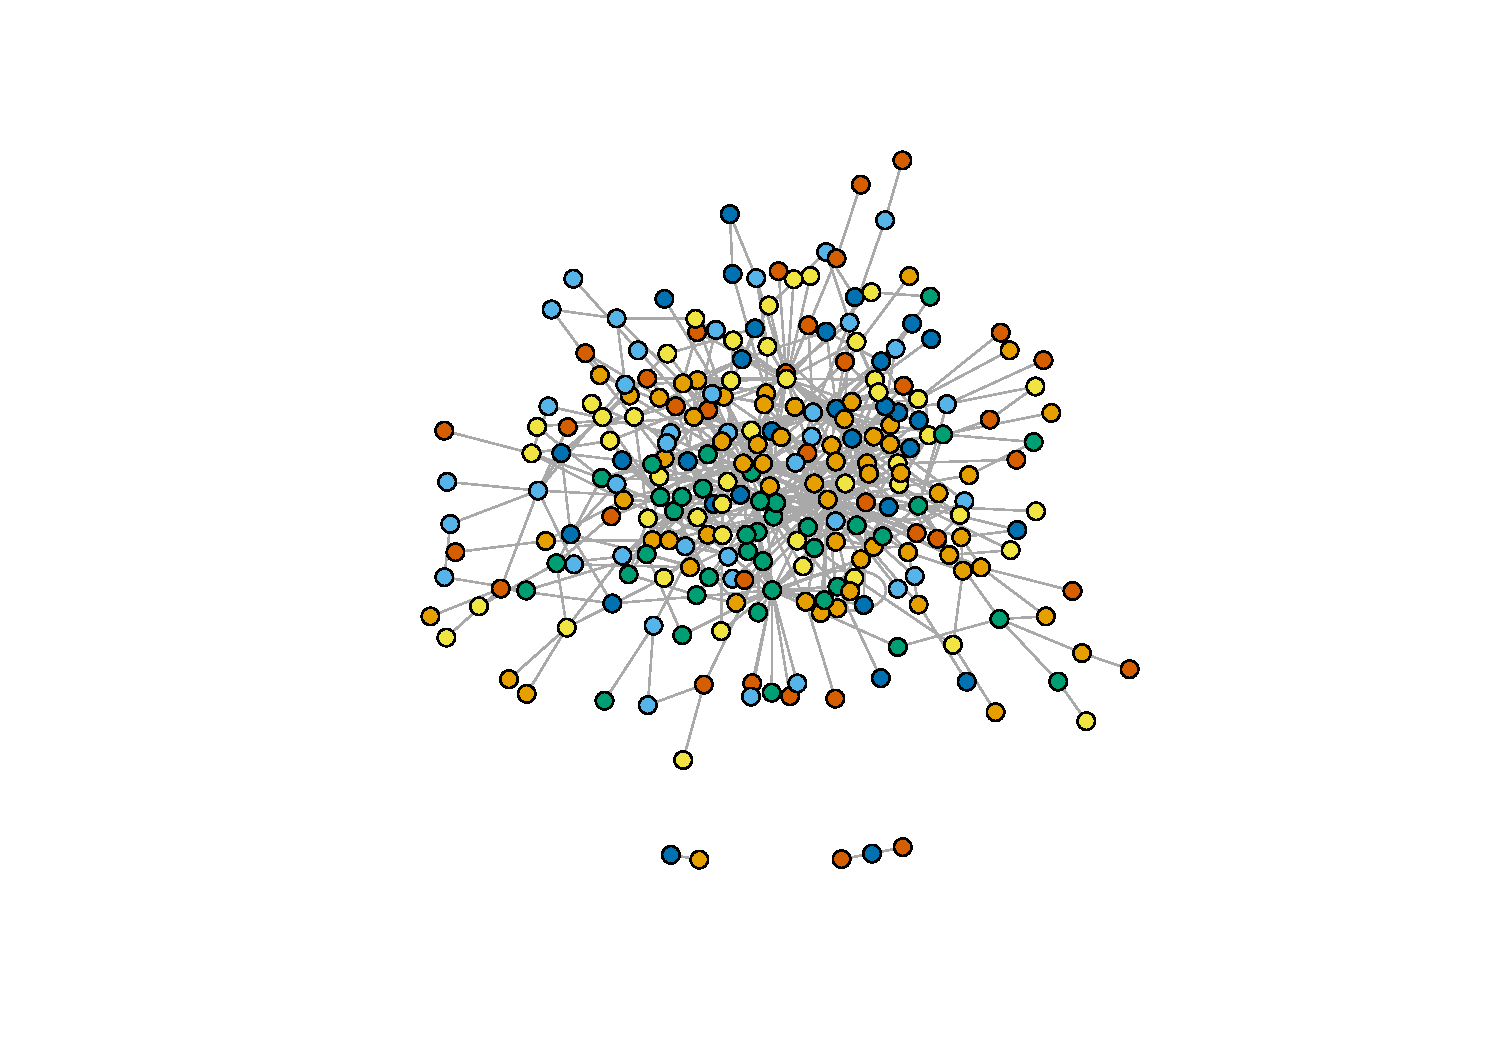
\includegraphics{presentation1_files/figure-beamer/unnamed-chunk-10-1.pdf}

\begin{verbatim}
## [1] 1
\end{verbatim}
\end{block}

\begin{block}{coreness and strength}
\protect\hypertarget{coreness-and-strength}{}
K-coreness is a measure of the centrality of a node within a network. It
is defined as the largest value of k such that the node belongs to a
subgraph of the network that is composed of nodes with at least degree
k. A node with a high k-coreness is considered to be more central and
influential within the network.

Strength is a measure of the total weight of the connections a node has
to other nodes in the network.
\end{block}

\begin{block}{sample network ( mu = 0.50 ): coreness and strength}
\protect\hypertarget{sample-network-mu-0.50-coreness-and-strength}{}
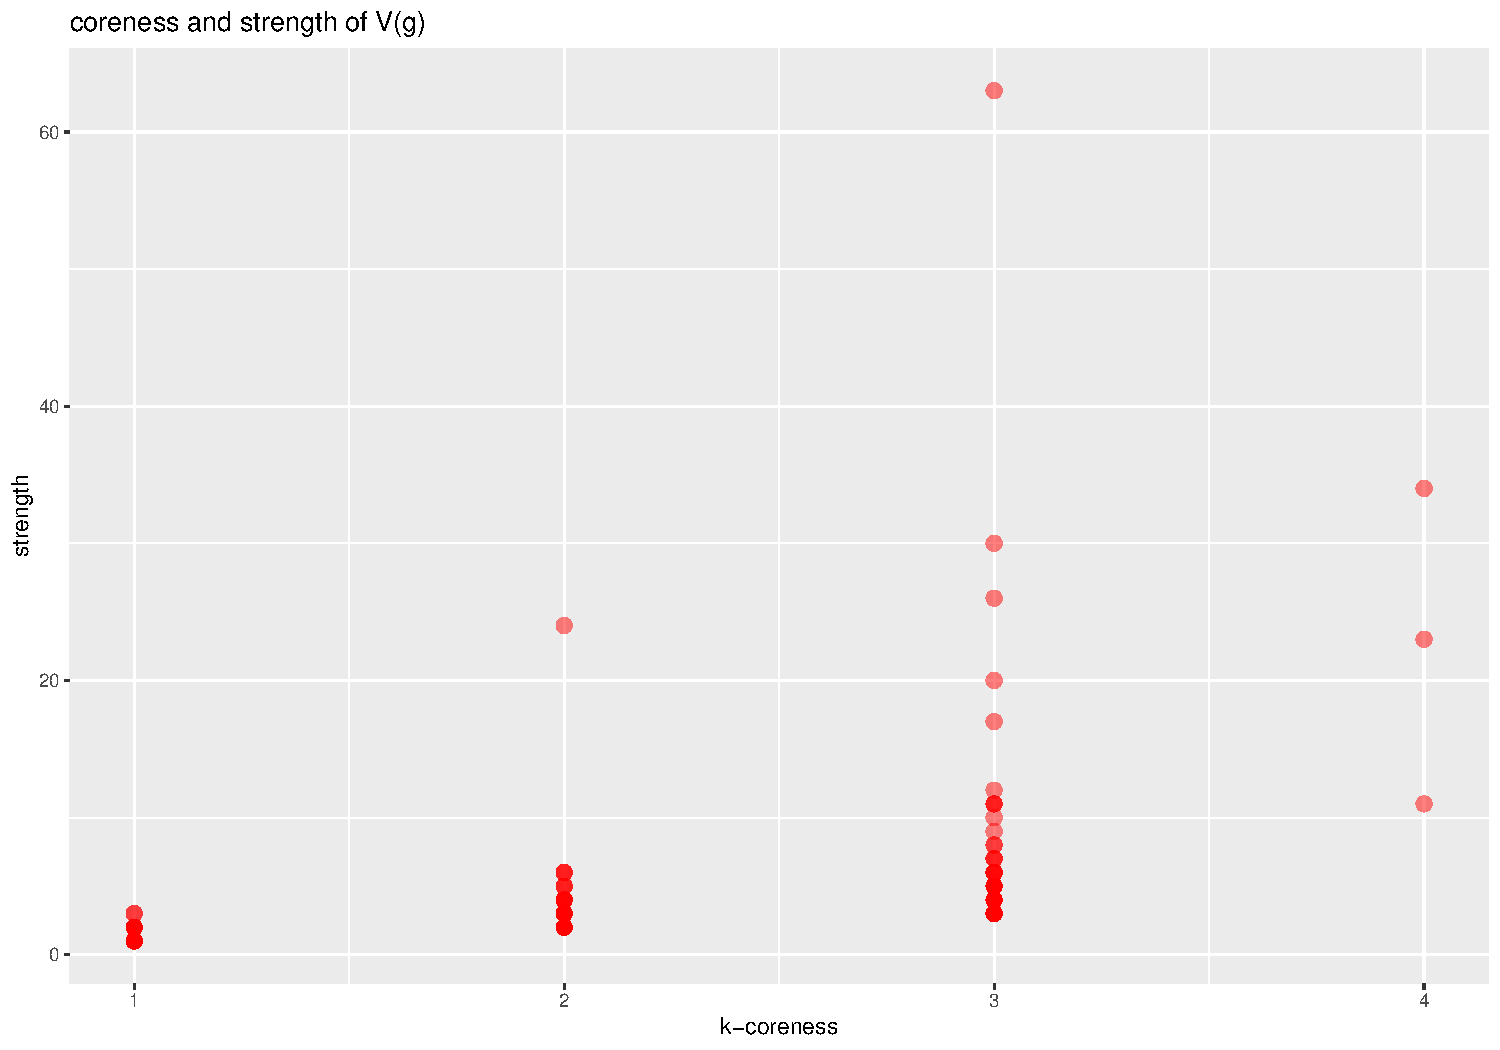
\includegraphics{presentation1_files/figure-beamer/unnamed-chunk-11-1.pdf}
\end{block}

\begin{block}{customized layout}
\protect\hypertarget{customized-layout}{}
\end{block}

\begin{block}{plot customized layout}
\protect\hypertarget{plot-customized-layout}{}
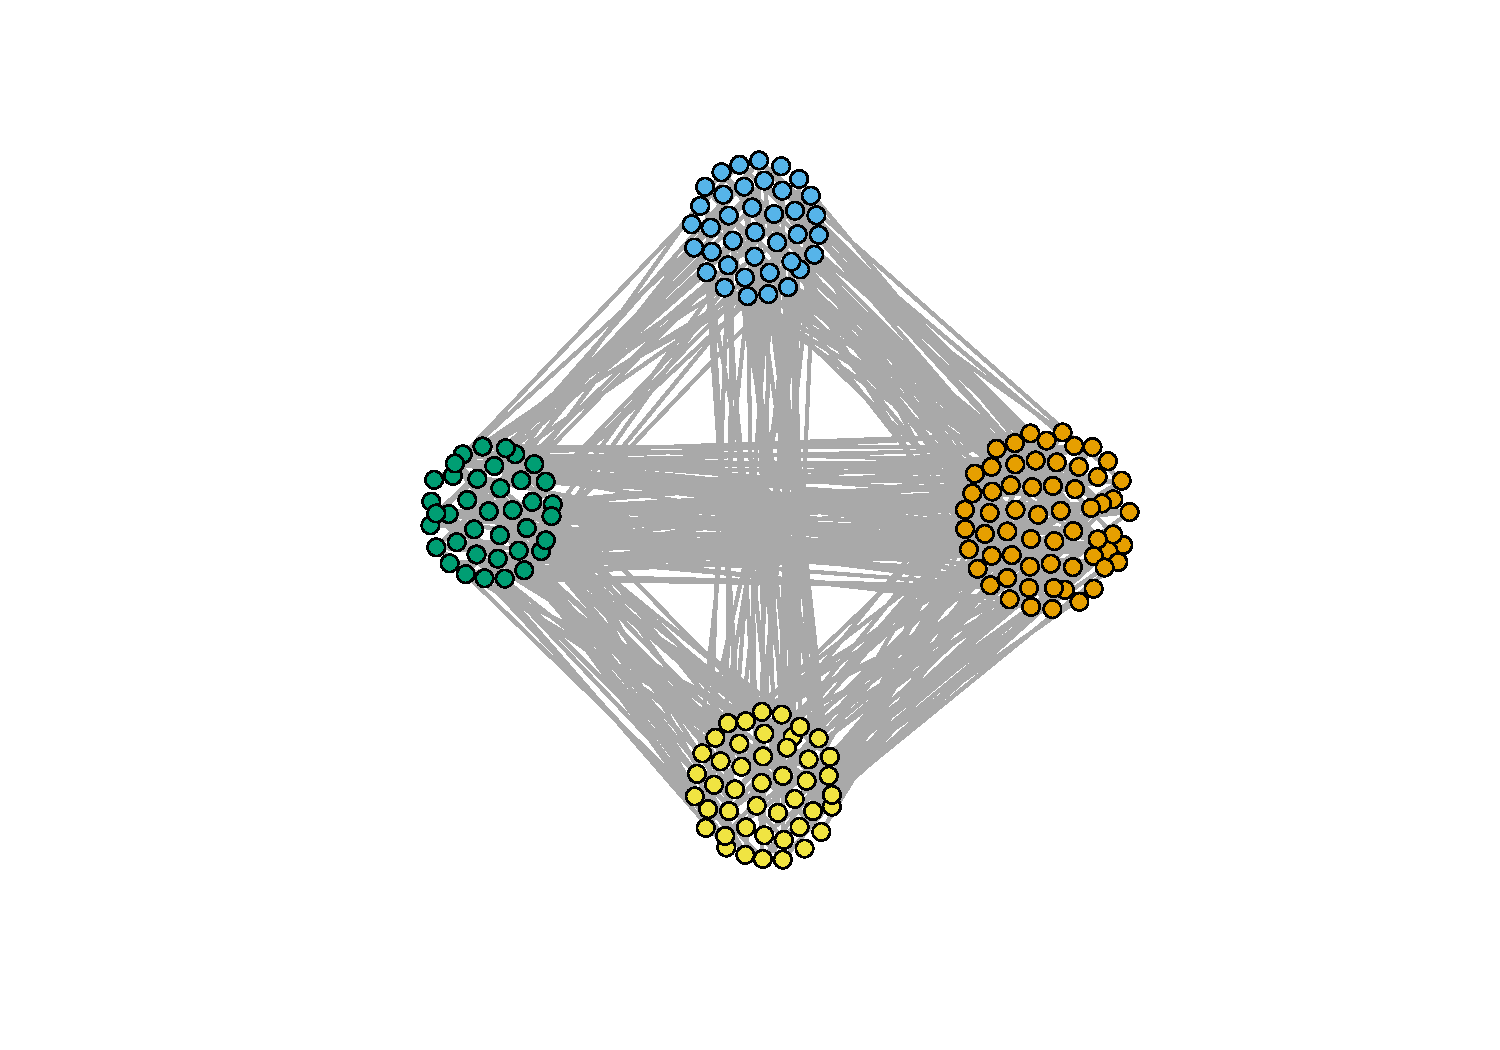
\includegraphics{presentation1_files/figure-beamer/unnamed-chunk-13-1.pdf}
\end{block}
\end{frame}

\begin{frame}{3 - unsupervised community detection}
\protect\hypertarget{unsupervised-community-detection}{}
\begin{block}{What is a community}
\protect\hypertarget{what-is-a-community}{}
the definition of `community' in network analysis depends on the context
and the researcher's goals. for example:

\begin{enumerate}
\item
  a community is a group of nodes that are more densely connected to
  each other than to the rest of the network.
\item
  a community is group of nodes that share certain characteristics, such
  as having similar properties
\item
  a community is a group of nodes that are more likely to interact with
  each other than with other nodes in the network.
\item
  \ldots{}
\end{enumerate}
\end{block}

\begin{block}{Modularity based community detection (1)}
\protect\hypertarget{modularity-based-community-detection-1}{}
\begin{itemize}
\item
  \textbf{Assumptions}:

  \begin{itemize}
  \item
    community is subset of nodes that are more densely connected to each
    other than to the rest of the network
  \item
    partition
  \item
    unsupervised (``true labels'' are not available - or not used for
    community detection)
  \end{itemize}
\end{itemize}
\end{block}

\begin{block}{Modularity based community detection (2)}
\protect\hypertarget{modularity-based-community-detection-2}{}
\begin{itemize}
\tightlist
\item
  \textbf{Definition of Modularity}: Given a network G partitioned into
  a number of communities Gi, modularity Q(G,Gi) is a function measuring
  the extent to which edge density is higher within than between
  communities. i.e.~a partition of G that maximises Q results in
  communities that have strong internal connections and weak connections
  with other communities
\end{itemize}

\emph{A partition with a higher modularity score indicates that the
edges within the partition are denser than the edges between partitions,
suggesting strong internal connections and weak connections with other
communities. \textbf{The optimal partition maximizes modularity}}
\end{block}

\begin{block}{Louvain community detection algorithm}
\protect\hypertarget{louvain-community-detection-algorithm}{}
Modularity optimization, by means of a hierarchical approach.

\begin{enumerate}
\item
  Initiates by partitioning the network so that each vertex is assigned
  to a single community.
\item
  Starting with a random vertex Vi, it computes the potential variation
  in modularity ΔQi j that would occur by aggregating Vi to each of its
  neighbours Vj.
\item
  If max(ΔQik) \textgreater{} 0 then, Vi is removed from its original
  community and aggregated to the neighbour Vk that maximises the gain.
\item
  The number of communities is thus reduced, and process is repeated
  sequentially for all other vertices until max(ΔQik)≤0 .
\end{enumerate}

As all methods based on modularity optimization it is biased by some
intrinsic limits

\begin{itemize}
\item
  greedy (find local optima)
\item
  Results depend on user-defined parameters
\item
  results depend on random initialisation and sequence of vrtices
\end{itemize}
\end{block}
\end{frame}

\begin{frame}[fragile]{4. robustness of results in \emph{fuzzy}
networks}
\protect\hypertarget{robustness-of-results-in-fuzzy-networks}{}
\begin{block}{a function to test the distribution of results}
\protect\hypertarget{a-function-to-test-the-distribution-of-results}{}
\end{block}

\begin{block}{sample network ( mu = 0.50 ): coreness and strength}
\protect\hypertarget{sample-network-mu-0.50-coreness-and-strength-1}{}
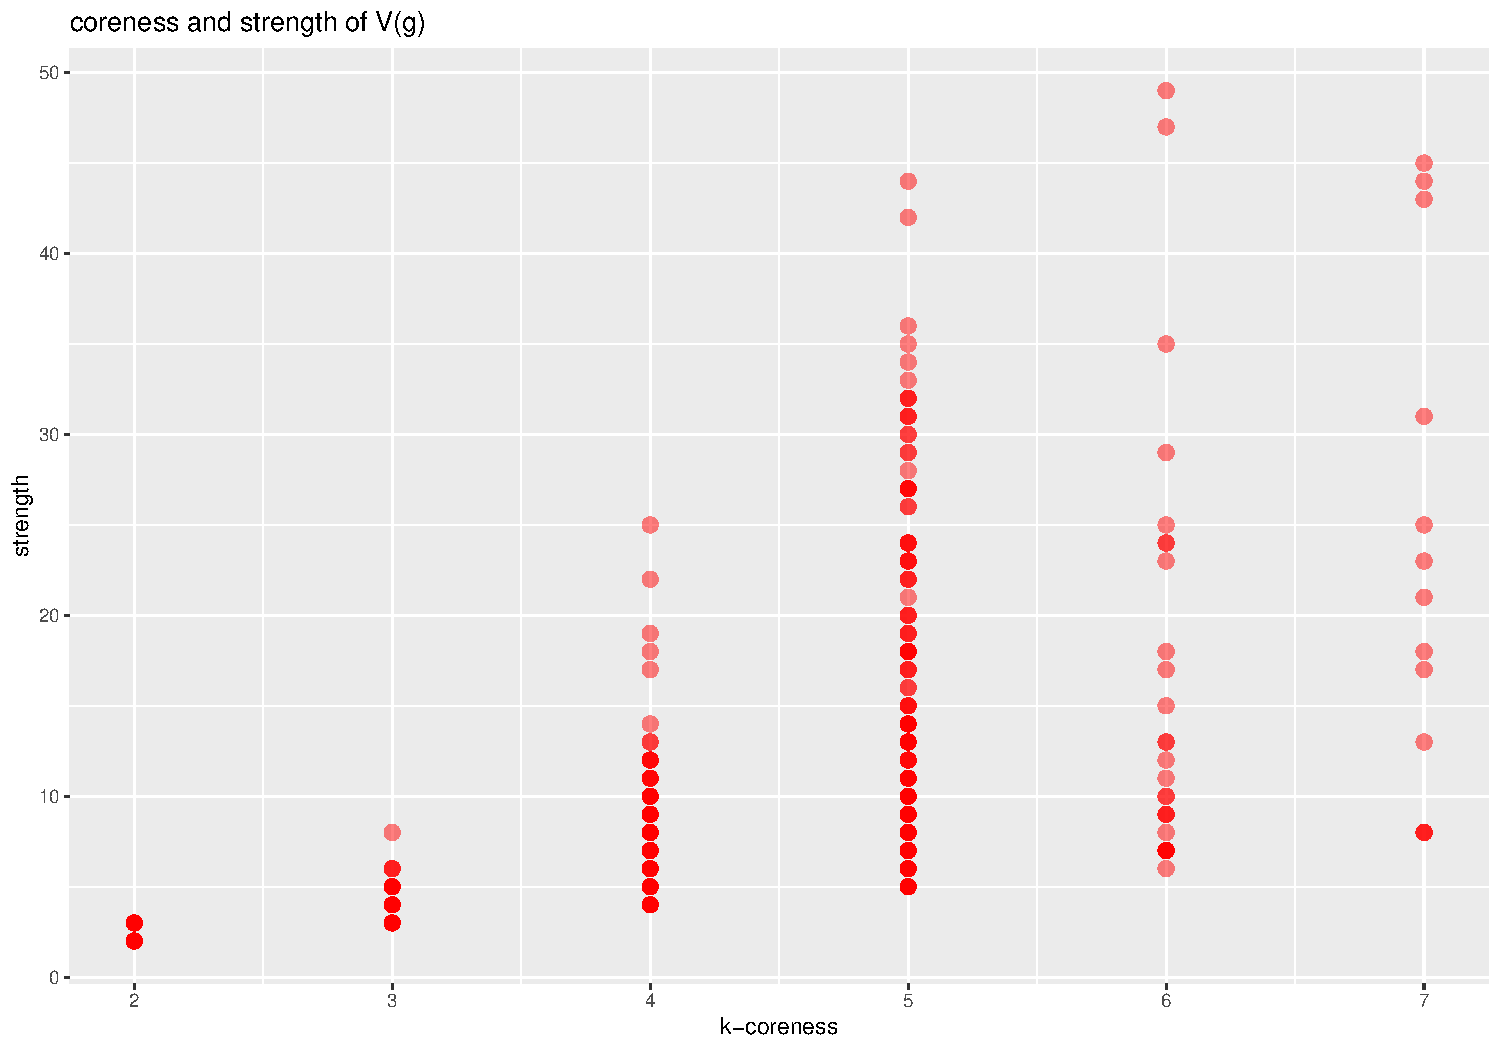
\includegraphics{presentation1_files/figure-beamer/unnamed-chunk-14-1.pdf}

\begin{verbatim}
## Warning: il pacchetto 'NMI' è stato creato con R versione 4.1.1
\end{verbatim}
\end{block}
\end{frame}

\begin{frame}[fragile]{Community detection: single trial}
\protect\hypertarget{community-detection-single-trial}{}
\begin{verbatim}
## [1] "Analysing  ./LFR_graphs/benchmark/FLR_benchmark_20.gml ..."
## [1] "Built-in communities:  37"
## [1] "Community detection results"
## [1] "Modularity:  0.724477609653802"
## [1] "Normalized Mutual Information 0.931891882472831"
## 
##  1  2  3  4  5  6  7  8  9 10 11 12 13 14 15 16 17 18 19 20 21 22 23 24 25 26 
## 43 53 29 21 25 27 30 53 31 40 43 24 40 41 33 47 40 26 31 24 49 36 24 20 43 42 
## 27 28 29 
## 25 36 23
\end{verbatim}
\end{frame}

\begin{frame}[fragile]{Community detection: repeated trials}
\protect\hypertarget{community-detection-repeated-trials}{}
\begin{verbatim}
## [1] "28 communities found"
## [1] "29 communities found"
## [1] "28 communities found"
## [1] "28 communities found"
## [1] "28 communities found"
## [1] "29 communities found"
## [1] "29 communities found"
## [1] "29 communities found"
## [1] "29 communities found"
## [1] "28 communities found"
\end{verbatim}

\begin{block}{Community detection: 1000 trials}
\protect\hypertarget{community-detection-1000-trials}{}
\end{block}

\begin{block}{results (1)}
\protect\hypertarget{results-1}{}
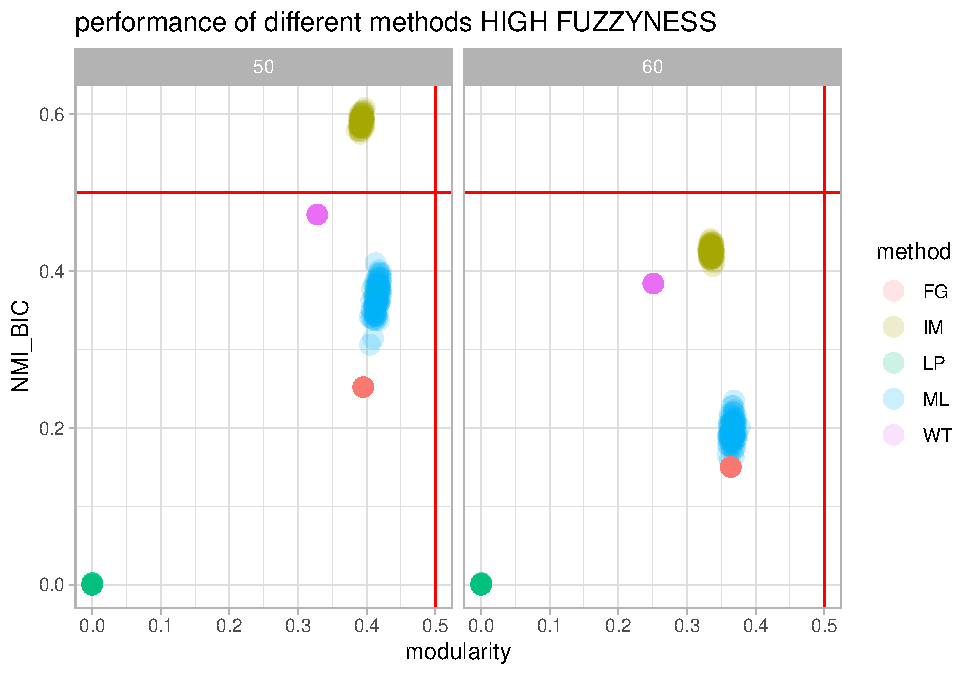
\includegraphics{presentation1_files/figure-beamer/unnamed-chunk-19-1.pdf}
\end{block}

\begin{block}{results (2)}
\protect\hypertarget{results-2}{}
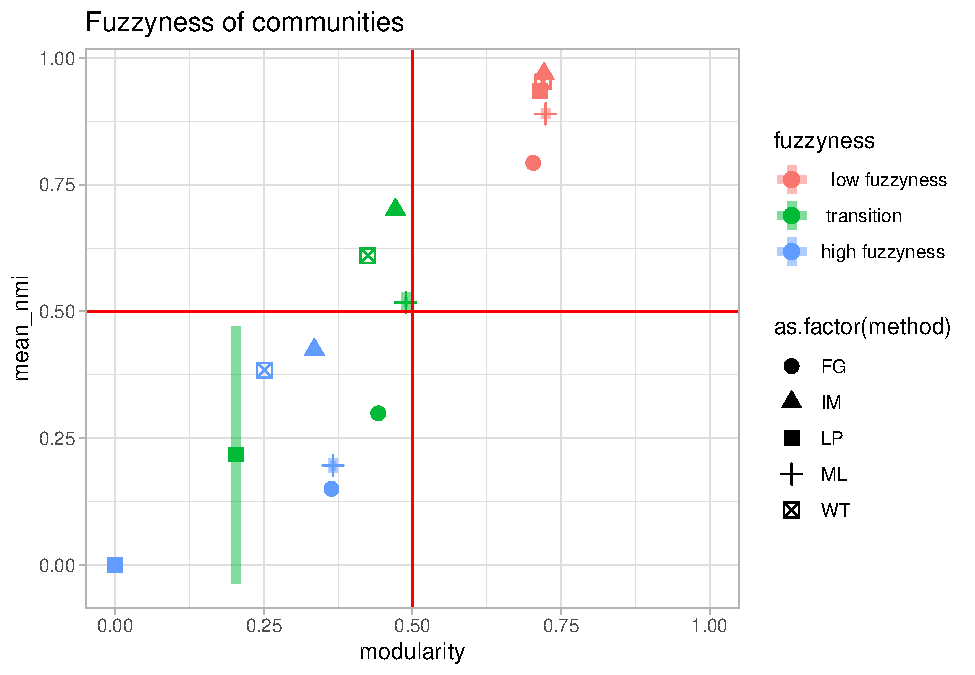
\includegraphics{presentation1_files/figure-beamer/unnamed-chunk-20-1.pdf}
\end{block}

\begin{block}{results (3)}
\protect\hypertarget{results-3}{}
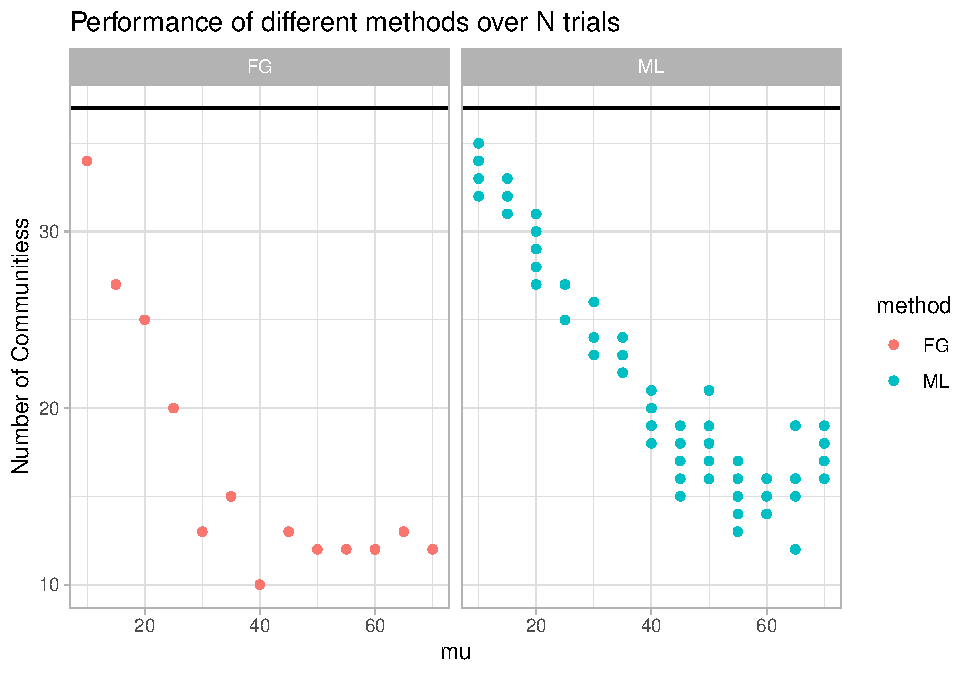
\includegraphics{presentation1_files/figure-beamer/unnamed-chunk-21-1.pdf}
\end{block}

\begin{block}{results (4)}
\protect\hypertarget{results-4}{}
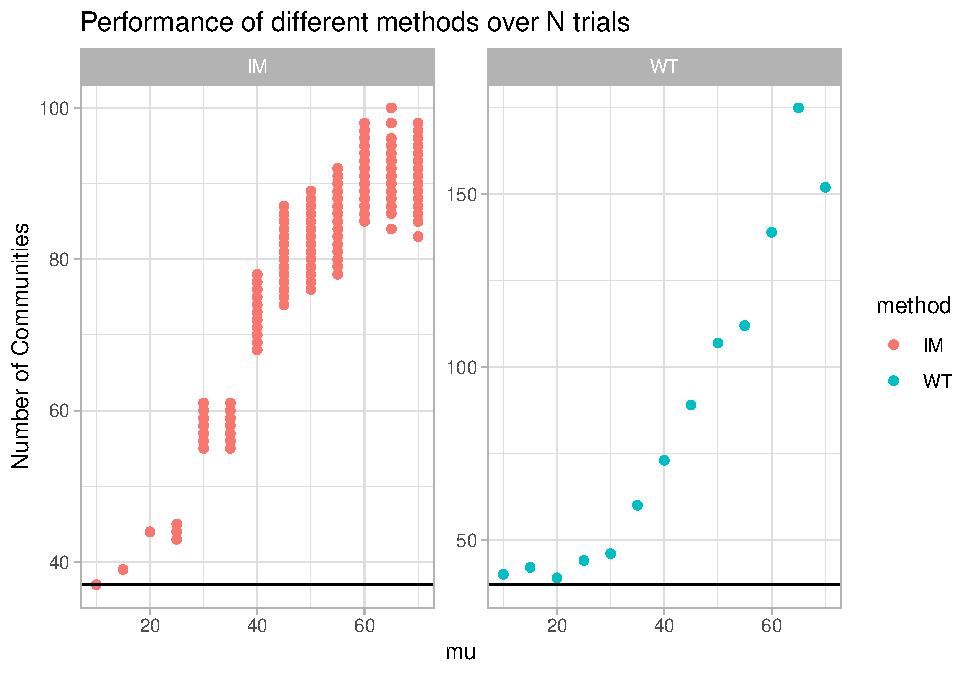
\includegraphics{presentation1_files/figure-beamer/unnamed-chunk-22-1.pdf}
\end{block}

\begin{block}{results (5)}
\protect\hypertarget{results-5}{}
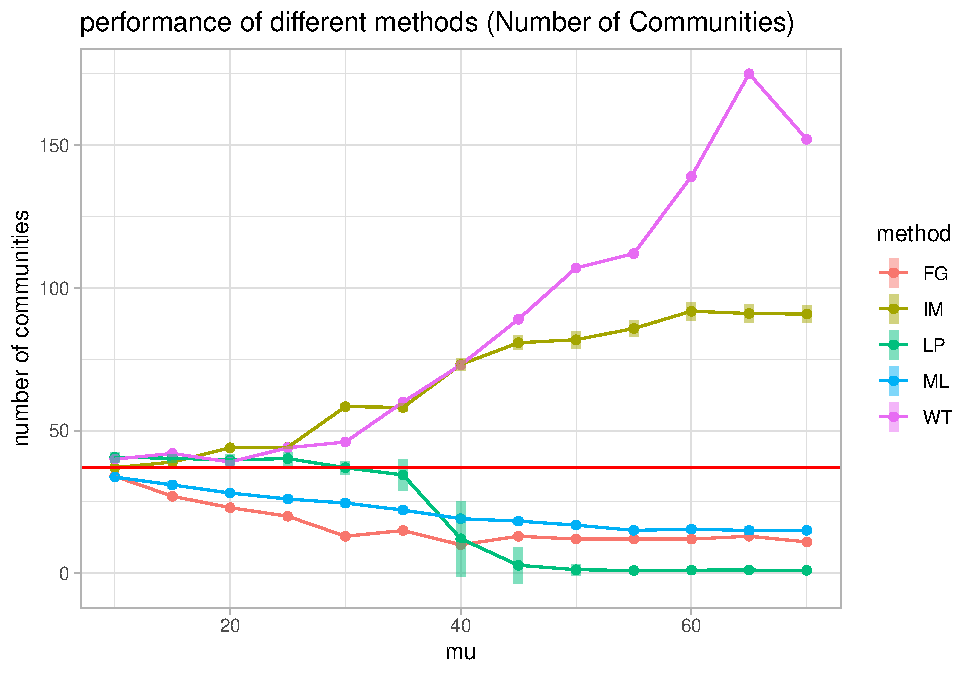
\includegraphics{presentation1_files/figure-beamer/unnamed-chunk-23-1.pdf}
\end{block}
\end{frame}

\begin{frame}[fragile]{5. consensus and ``robustness of membership''}
\protect\hypertarget{consensus-and-robustness-of-membership}{}
\begin{block}{inspired by 'random forrest'' algorithm}
\protect\hypertarget{inspired-by-random-forrest-algorithm}{}
Random Forest is an ensemble machine learning algorithm that combines
the results produced by multiple independent instances of `regression
tree' (or `decision tree') to obtain predictive performance than could
be obtained from any of the `trees' alone.

The algorithm builds N = 500 trees, each based on a randomly selected
subset of features from the training dataset. The final prediction is
made by averaging the predictions (or selecting the mode) of all the N
trees.

\textbf{note}: Random Forest is a \emph{supervised} algorithm (community
detection is \emph{unsupervised})
\end{block}

\begin{block}{Consensus community detection (CCD)}
\protect\hypertarget{consensus-community-detection-ccd}{}
CCD can be used to enhance both the stability and the accuracy of the
resulting partitions, reducing dependence on user-defined parameters and
random initialization

Principles:

\begin{verbatim}
-   **Independent trials**

-   **Consensus**

-   **Pruning**
\end{verbatim}
\end{block}

\begin{block}{Consensus community detection (CCD)}
\protect\hypertarget{consensus-community-detection-ccd-1}{}
\textbf{Independent trials:} The Louvain community detection algorithm
is repeated Ni times, and at each iteration only a part of the
information in the network is used i.e.~a randomly chosen fraction α of
edges is assigned a weight W0 (small, but non-zero). The resulting
network is not losing connectivity, but edges associated with W0 are
more likely to be assigned to different community at each iteration
\end{block}

\begin{block}{Consensus community detection (CCD)}
\protect\hypertarget{consensus-community-detection-ccd-2}{}
\textbf{Consensus}: the consensus algorithm counts how many times a pair
of vertices Vi and Vj are assigned to the same community and assigns a
\textbf{\emph{proportion of membership}} PVij ∈ {[}0,1{]}.

Vertices that are strongly connected to one another are always assigned
to the same community and have PVij = 1; lower values of Pvij indicate
that the vertex is not strongly connected to its neighbors, and it may
be assigned to two or more communities with some degree of confidence.
\end{block}

\begin{block}{Consensus community detection (CCD)}
\protect\hypertarget{consensus-community-detection-ccd-3}{}
\textbf{Pruning}: The algorithm creates a meta-community labelled as
``community 0'' defined by regular equivalence (i.e.~vertices covering
the same ``marginal'' role in the network):

\begin{itemize}
\tightlist
\item
  Vertices with max(Pvij) \textless{} 0.5
\item
  Trivially small communities of size Scommunity \textless{} Scmin ,
\item
  Trivially small communities of weight Wcommunity \textless{} Wcmin
\end{itemize}
\end{block}

\begin{block}{CCD parameters}
\protect\hypertarget{ccd-parameters}{}
Independent trials

\begin{itemize}
\item
  - N repetitions: independent repetitions of the whole procedure
\item
  - N trials: independent trials of modularity based community detection
\end{itemize}

Consensus

\begin{itemize}
\item
  Alpha: fraction of edges that is assigned a weight W0. \emph{default
  0.05}
\item
  Epsilon: to set the appropriate value of W0 = min(Wi * Epsilon)
  \emph{default 0.01}
\item
  Resolution: parameter of Louvain Community Detection \emph{default
  1.0}
\item
  P\_threshold: proportion of membership threshold \emph{default 0.5}
\end{itemize}
\end{block}

\begin{block}{simulation plan (1)}
\protect\hypertarget{simulation-plan-1}{}
\end{block}

\begin{block}{simulation plan (2)}
\protect\hypertarget{simulation-plan-2}{}
We simulate several LFR networks setting different parameters hat
reproduce some of the key structural features of a network of interest
(labour market network of Friuli Venezia Giulia)

\begin{itemize}
\item
  N=1000
\item
  Average degree = 10
\item
  Community size min = 20 max = 50 Tau1 = 2
\item
  Tau2 = 3
\item
  mu \{ 0.1, 0.2, \ldots. 0.9 \}
\item
  Mu is the crucial parameter for our test, as it governs the fuzziness
  of communities.
\end{itemize}
\end{block}

\begin{block}{results (1)}
\protect\hypertarget{results-1-1}{}
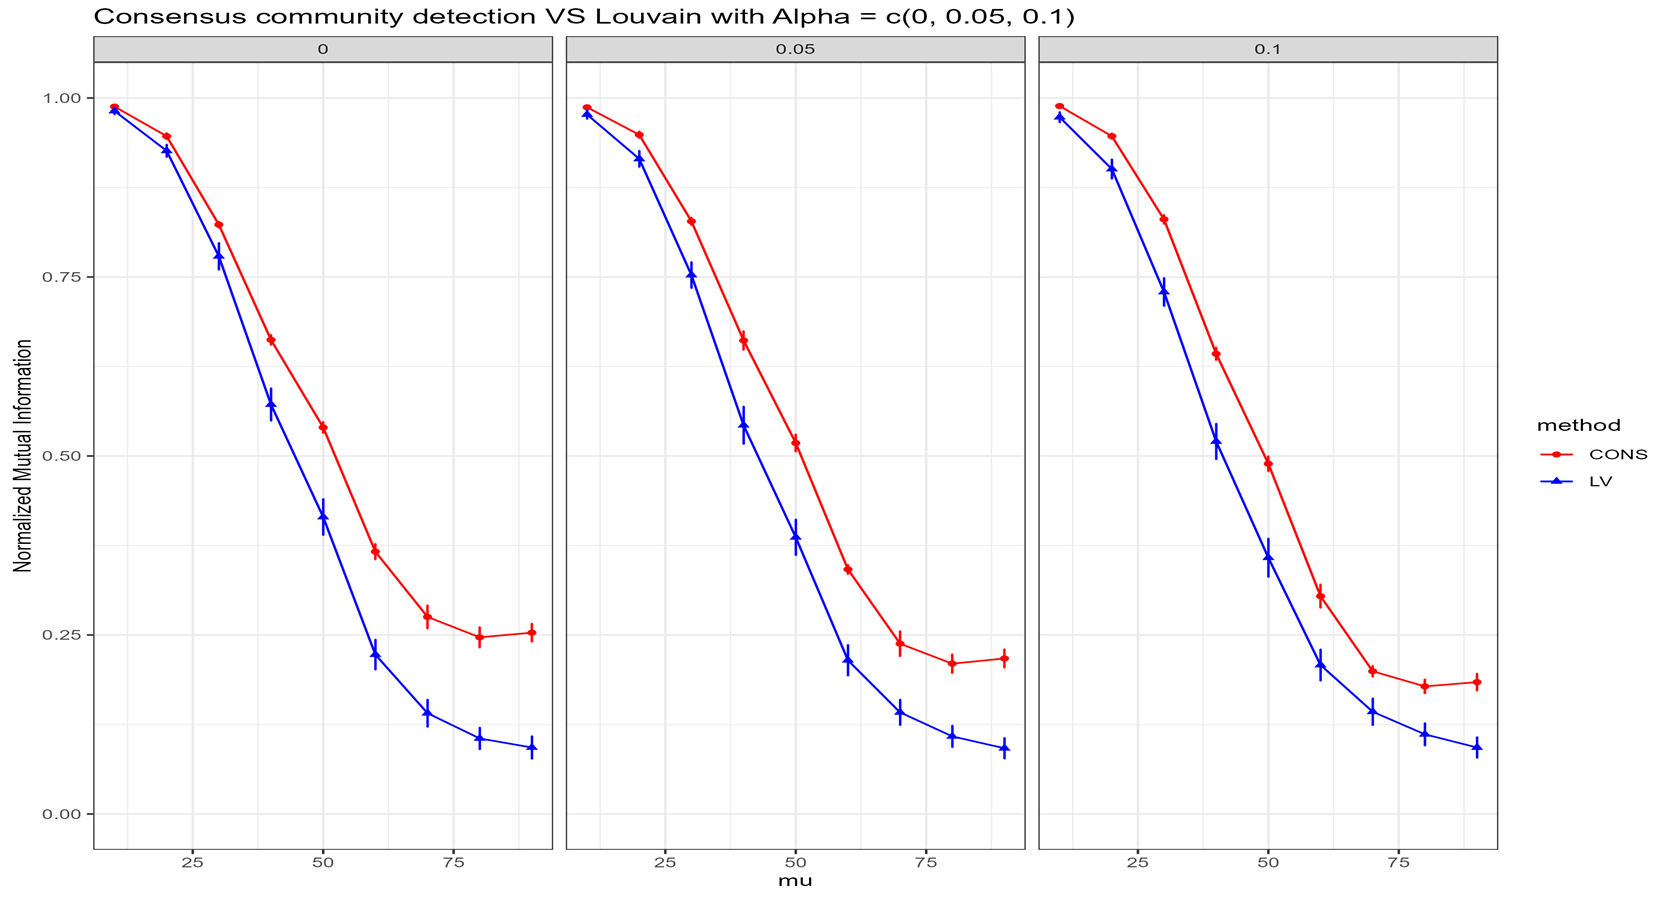
\includegraphics[width=7.91667in,height=4.39583in]{images/paste-89AB04A9.png}
\end{block}

\begin{block}{results (2)}
\protect\hypertarget{results-2-1}{}
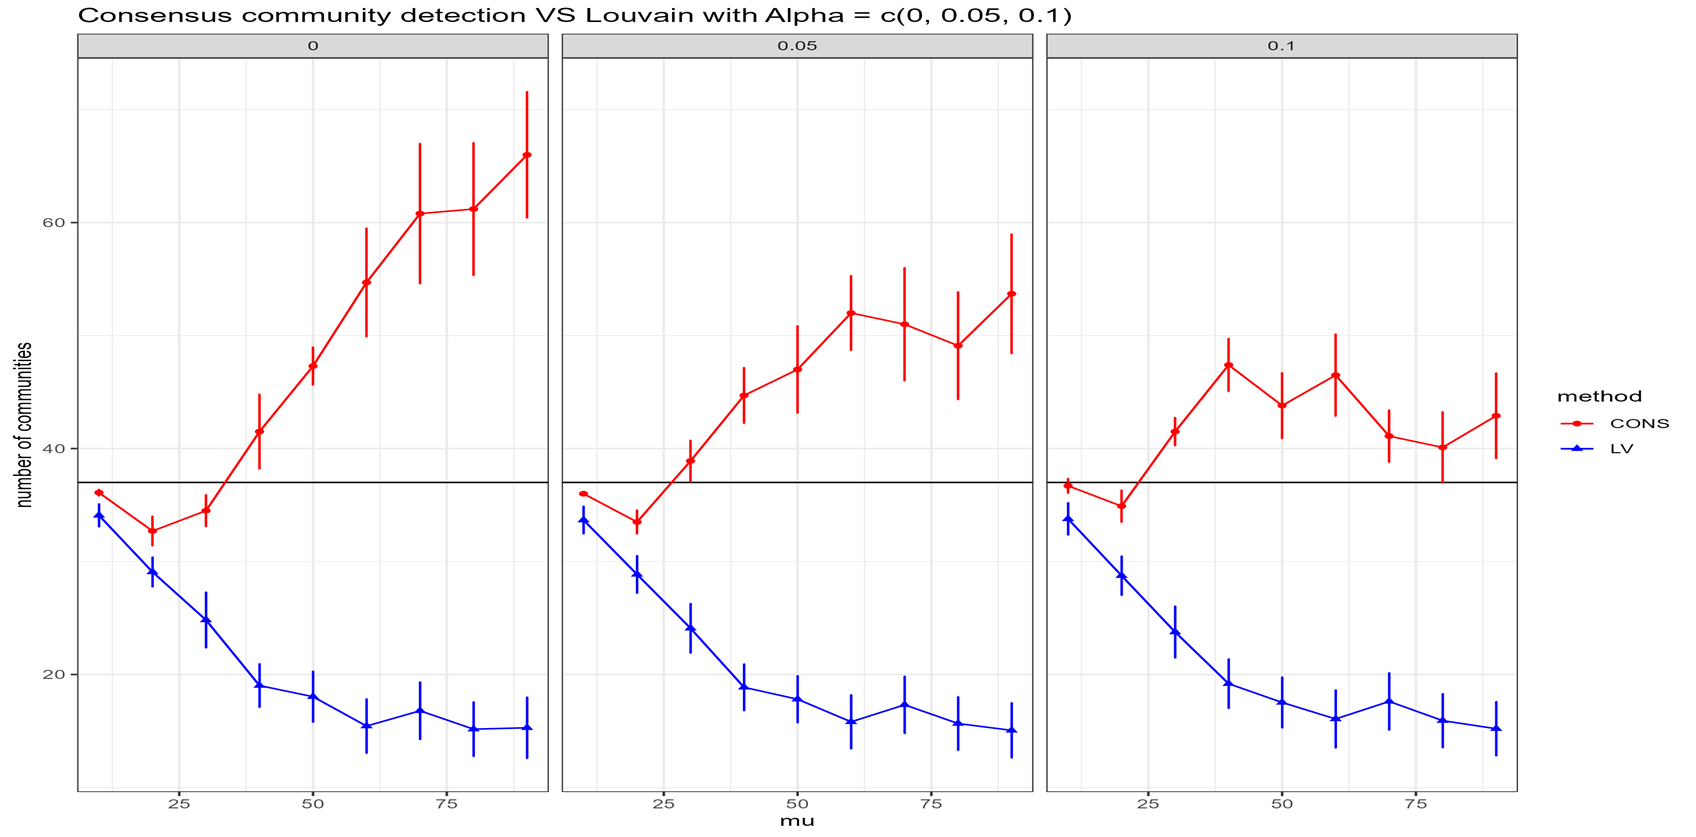
\includegraphics[width=6.89583in,height=4.5in]{images/paste-F8669B18.png}
\end{block}

\begin{block}{results (3)}
\protect\hypertarget{results-3-1}{}
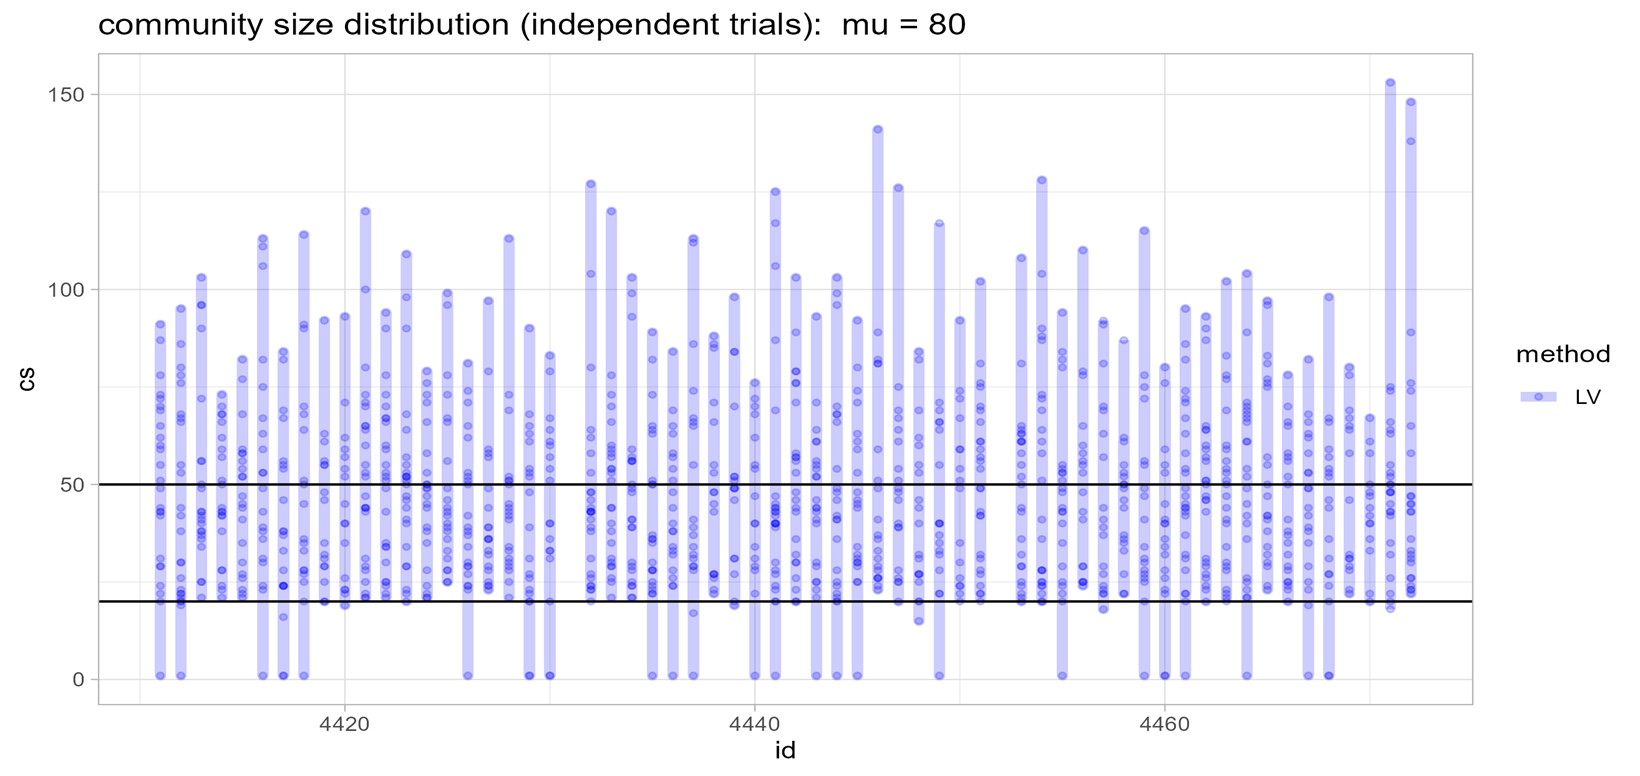
\includegraphics[width=5.94792in,height=3.77083in]{images/paste-657043E9.png}
\end{block}
\end{frame}

\begin{frame}{6. sample results in a ``labour market network''}
\protect\hypertarget{sample-results-in-a-labour-market-network}{}
\begin{block}{Coreness and strength}
\protect\hypertarget{coreness-and-strength-1}{}
\end{block}

\begin{block}{Communities}
\protect\hypertarget{communities}{}
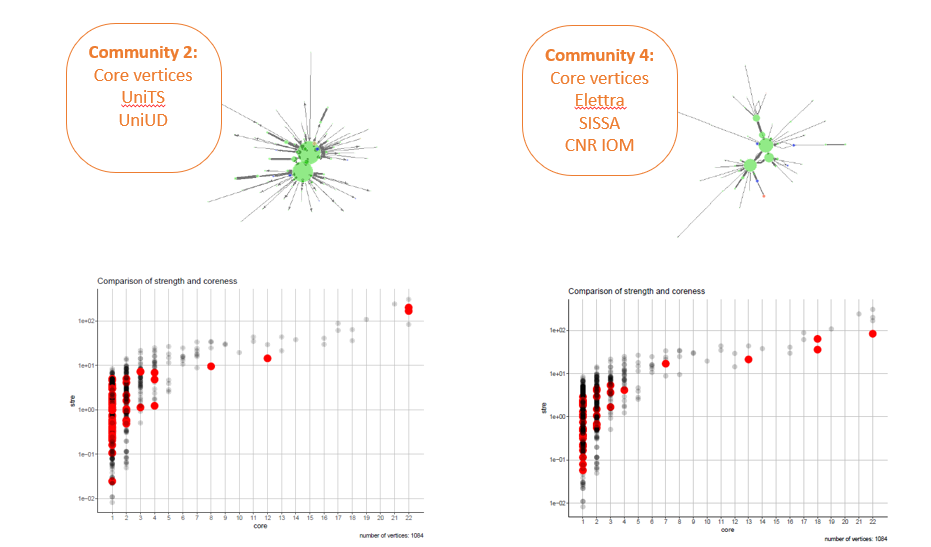
\includegraphics[width=5.9375in,height=\textheight]{images/paste-484EE1EF.png}
\end{block}

\begin{block}{Community ``0''}
\protect\hypertarget{community-0}{}
Community 0 is a community of regular equivalent organizations or
organisation whose membership is strongly dependent on the random
initialisation of the community detection algorithm

\begin{itemize}
\item
  Disconnected components
\item
  Communities identified by consensus algorithm that fall below
  thresholds of size of weight
\item
  Nodes that are assigned to different commuities at each run of Louvain
  community detection
\end{itemize}
\end{block}

\begin{block}{Community ``0''}
\protect\hypertarget{community-0-1}{}
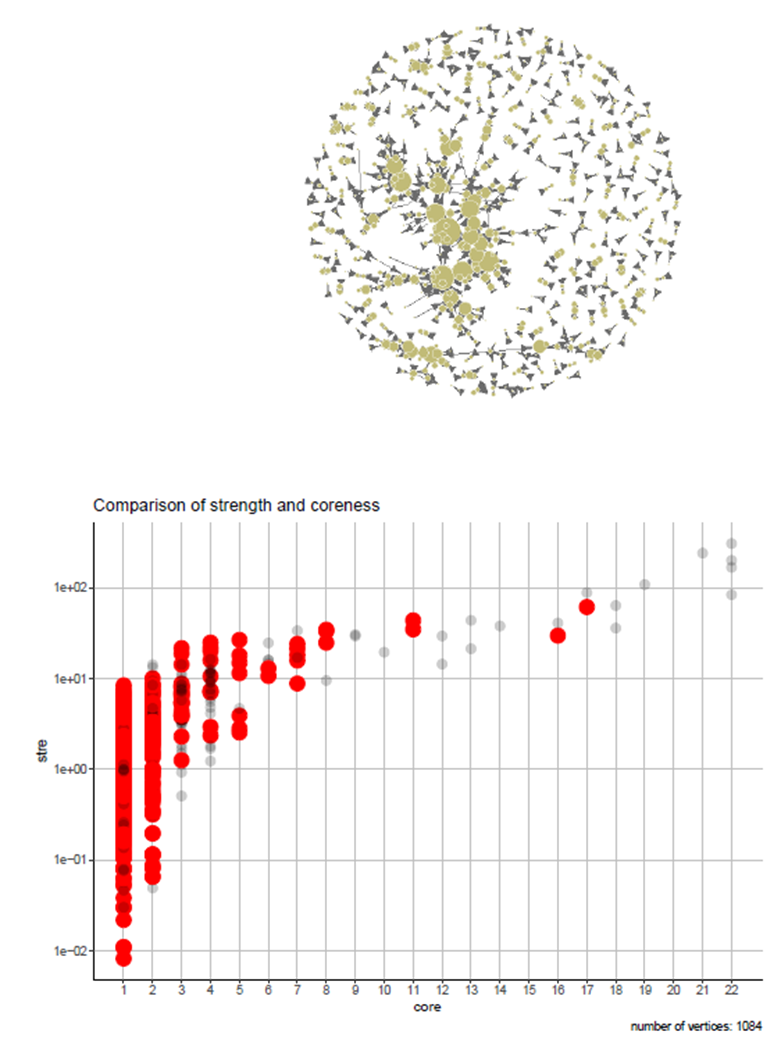
\includegraphics[width=4.47917in,height=\textheight]{images/paste-91D29A70.png}
\end{block}
\end{frame}

\end{document}
